
%%%%%%%%%%%%%%%%%%%%%%%%%%%%%%%%%%%%%%%%%%%%%%%%%%%%%%%%%%%%%%%%%%%%%
%% This is a (brief) model paper using the achemso class
%% The document class accepts keyval options, which should include
%% the target journal and optionally the manuscript type.
%%%%%%%%%%%%%%%%%%%%%%%%%%%%%%%%%%%%%%%%%%%%%%%%%%%%%%%%%%%%%%%%%%%%%
\documentclass[journal=acsnano,manuscript=article]{achemso}

%%%%%%%%%%%%%%%%%%%%%%%%%%%%%%%%%%%%%%%%%%%%%%%%%%%%%%%%%%%%%%%%%%%%%
%% Place any additional packages needed here.  Only include packages
%% which are essential, to avoid problems later. Do NOT use any
%% packages which require e-TeX (for example etoolbox): the e-TeX
%% extensions are not currently available on the ACS conversion
%% servers.
%%%%%%%%%%%%%%%%%%%%%%%%%%%%%%%%%%%%%%%%%%%%%%%%%%%%%%%%%%%%%%%%%%%%%
\usepackage[version=3]{mhchem} % Formula subscripts using \ce{}
\usepackage[T1]{fontenc}       % Use modern font encodings
\usepackage{graphicx}
\usepackage{subcaption}
\usepackage{fixltx2e}
\usepackage{color}

%%%%%%%%%%%%%%%%%%%%%%%%%%%%%%%%%%%%%%%%%%%%%%%%%%%%%%%%%%%%%%%%%%%%%
%% If issues arise when submitting your manuscript, you may want to
%% un-comment the next line.  This provides information on the
%% version of every file you have used.
%%%%%%%%%%%%%%%%%%%%%%%%%%%%%%%%%%%%%%%%%%%%%%%%%%%%%%%%%%%%%%%%%%%%%
%%\listfiles

%%%%%%%%%%%%%%%%%%%%%%%%%%%%%%%%%%%%%%%%%%%%%%%%%%%%%%%%%%%%%%%%%%%%%
%% Place any additional macros here.  Please use \newcommand* where
%% possible, and avoid layout-changing macros (which are not used
%% when typesetting).
%%%%%%%%%%%%%%%%%%%%%%%%%%%%%%%%%%%%%%%%%%%%%%%%%%%%%%%%%%%%%%%%%%%%%
\newcommand*\mycommand[1]{\texttt{\emph{#1}}}
\newcommand\crule[3][black]{\textcolor{#1}{\rule{#2}{#3}}}
\newcommand{\angstrom}{\textup{\AA}}
\graphicspath{{snapshots/},{flexible/},{rigid/}}

%%%%%%%%%%%%%%%%%%%%%%%%%%%%%%%%%%%%%%%%%%%%%%%%%%%%%%%%%%%%%%%%%%%%%
%% Meta-data block
%% ---------------
%% Each author should be given as a separate \author command.
%%
%% Corresponding authors should have an e-mail given after the author
%% name as an \email command. Phone and fax numbers can be given
%% using \phone and \fax, respectively; this information is optional.
%%
%% The affiliation of authors is given after the authors; each
%% \affiliation command applies to all preceding authors not already
%% assigned an affiliation.
%%
%% The affiliation takes an option argument for the short name.  This
%% will typically be something like "University of Somewhere".
%%
%% The \altaffiliation macro should be used for new address, etc.
%% On the other hand, \alsoaffiliation is used on a per author basis
%% when authors are associated with multiple institutions.
%%%%%%%%%%%%%%%%%%%%%%%%%%%%%%%%%%%%%%%%%%%%%%%%%%%%%%%%%%%%%%%%%%%%%
\author{Lisa E. Felberg}
\affiliation{Department of Chemical and Biomolecular Engineering, University of California Berkeley, Berkeley, California 94720, USA}
\author{Luis A. Ruiz Pestana}
\affiliation{Chemical Sciences Division, Lawrence Berkeley National Labs, Berkeley, California 94720, USA}
\author{Teresa Head-Gordon}
\affiliation{Department of Chemical and Biomolecular Engineering, University of California Berkeley, Berkeley, California 94720, USA}
\alsoaffiliation{Chemical Sciences Division, Lawrence Berkeley National Labs, Berkeley, California 94720, USA}
\alsoaffiliation{Department of Chemistry, University of California Berkeley, Berkeley, California 94720, USA}
\alsoaffiliation{Department of Bioengineering, University of California Berkeley, Berkeley, California 94720, USA}
\email{thg@berkeley.edu}

%%%%%%%%%%%%%%%%%%%%%%%%%%%%%%%%%%%%%%%%%%%%%%%%%%%%%%%%%%%%%%%%%%%%%
%% The document title should be given as usual. Some journals require
%% a running title from the author: this should be supplied as an
%% optional argument to \title.
%%%%%%%%%%%%%%%%%%%%%%%%%%%%%%%%%%%%%%%%%%%%%%%%%%%%%%%%%%%%%%%%%%%%%
\title[confinement]
  {Confinement}

%%%%%%%%%%%%%%%%%%%%%%%%%%%%%%%%%%%%%%%%%%%%%%%%%%%%%%%%%%%%%%%%%%%%%
%% Some journals require a list of abbreviations or keywords to be
%% supplied. These should be set up here, and will be printed after
%% the title and author information, if needed.
%%%%%%%%%%%%%%%%%%%%%%%%%%%%%%%%%%%%%%%%%%%%%%%%%%%%%%%%%%%%%%%%%%%%%
\abbreviations{IR,NMR,UV}
\keywords{confinement, 2D water}

%%%%%%%%%%%%%%%%%%%%%%%%%%%%%%%%%%%%%%%%%%%%%%%%%%%%%%%%%%%%%%%%%%%%%
%% The manuscript does not need to include \maketitle, which is
%% executed automatically.
%%%%%%%%%%%%%%%%%%%%%%%%%%%%%%%%%%%%%%%%%%%%%%%%%%%%%%%%%%%%%%%%%%%%%
\begin{document}

%%%%%%%%%%%%%%%%%%%%%%%%%%%%%%%%%%%%%%%%%%%%%%%%%%%%%%%%%%%%%%%%%%%%%
%% The "tocentry" environment can be used to create an entry for the
%% graphical table of contents. It is given here as some journals
%% require that it is printed as part of the abstract page. It will
%% be automatically moved as appropriate.
%%%%%%%%%%%%%%%%%%%%%%%%%%%%%%%%%%%%%%%%%%%%%%%%%%%%%%%%%%%%%%%%%%%%%
\begin{tocentry}

Some journals require a graphical entry for the Table of Contents.
This should be laid out ``print ready'' so that the sizing of the
text is correct.

Inside the \texttt{tocentry} environment, the font used is Helvetica
8\,pt, as required by \emph{Journal of the American Chemical
Society}.

The surrounding frame is 9\,cm by 3.5\,cm, which is the maximum
permitted for  \emph{Journal of the American Chemical Society}
graphical table of content entries. The box will not resize if the
content is too big: instead it will overflow the edge of the box.

This box and the associated title will always be printed on a
separate page at the end of the document.

\end{tocentry}

%%%%%%%%%%%%%%%%%%%%%%%%%%%%%%%%%%%%%%%%%%%%%%%%%%%%%%%%%%%%%%%%%%%%%
%% The abstract environment will automatically gobble the contents
%% if an abstract is not used by the target journal.
%%%%%%%%%%%%%%%%%%%%%%%%%%%%%%%%%%%%%%%%%%%%%%%%%%%%%%%%%%%%%%%%%%%%%
\begin{abstract}
  
\end{abstract}

%%%%%%%%%%%%%%%%%%%%%%%%%%%%%%%%%%%%%%%%%%%%%%%%%%%%%%%%%%%%%%%%%%%%%
%% Start the main part of the manuscript here.
%%%%%%%%%%%%%%%%%%%%%%%%%%%%%%%%%%%%%%%%%%%%%%%%%%%%%%%%%%%%%%%%%%%%%
\section{Introduction}
The properties and phase behavior of water under nanoconfinement are remarkably different than those in bulk, which has important implications for nanotechnological applications and a myriad of biological processes \cite{Lucent2007, Holt2006, Levinger2002, Nair2012}. Driven by the pursuit of understanding the anomalous phase behavior of confined water, topics such as low-dimensional ice formation \cite{Algara-Siller2015, Zhou2015, Koga2001}, unconventional phase transitions \cite{Mochizuki2015,Han2010,Giovambattista2009,Zhu2015}, and hydrophobic evaporation or dewetting \cite{Sharma2012,Altabet2017,Head-Gordon2008,Hummer2001}, have been extensively studied over the last decade. Most of the studies, however, have focused on rigid confinement. Only a handful of papers have investigated water confined under flexible surfaces \cite{Algara-Siller2015,Deshmukh2014,Altabet2017}, and none have addressed systematically the phase behavior of water under those conditions. Studying flexible confinement is critical to understand the role that confinement plays on biological processes where soft interfaces are ubiquitous, or to exploit confinement effects in engineered systems where 2D materials, inherently flexible, are pervasively employed \cite{Deng2016}. In terms of 2D materials, the epitome is perhaps graphene \cite{Geim2007}, a highly flexible two-dimensional carbon allotrope \cite{Wei2013,Fasolino2007}, that has become a paradigmatic example of hydrophobic confining surface. The question we aim to answer here is whether the phase behavior of water mapped under rigid confinement can be extended to the more relevant scenario of flexible confinement. We focus on ambient conditions of temperature and pressure that are relevant in most practical applications.
	
	When water is confined under slit nanocapillaries it adopts a multi-layered structure characterized by strong density fluctuations along the direction of confinement. The effect of the confining surfaces persists at short range, ca. 5 \r A \cite{Cicero2008,Chialvo2016}, therefore multi-layered states of only up to three layers can be stable under planar confinement. In fact, trilayers of ice \cite{Algara-Siller2015,Satarifard2017,Zhu2015} and liquid water \cite{Giovambattista2009,Qiu2015} have been reported, but nothing beyond that. The tendency to form layered structures makes the commensurability between the confinement distance and the density of water an important aspect. In an incommensurate configuration, the density of water is too high or two low, all other control parameters constant, for the water molecules to form full layers of whatever phase is lower in energy under those thermodynamic conditions. A recent study found that oscillations in the shear viscosity of confined water of several orders of magnitude occur over small variations in the confinement distance (under 1 \r A) due to transitions between incommensurate and commensurate states \cite{Neek-Amal2016}. Phase transitions can also be triggered upon changes in commensurability. Giovambattista et al. found a transition between a bilayer liquid (BL) and a trilayer heterogeneous fluid (THF) upon increasing the density of water while keeping the confinement distance constant between 8 \r A and 9 \r A. The THF phase was characterized by highly ordered layers close to the confining surfaces and a disordered middle layer. When the confinement distance was kept at 6 \r A, a transition between THF and bilayer ice (BI) occurred upon decompression instead. Commensurability also plays a critical role on the formation of crystalline configurations with long-range in-plane order such as ice \cite{Satarifard2017,Chen2017,Corsetti2016}. For commensurate configurations at room temperature, multi-layered ice can form under confinement at pressures in the order of several GPa \cite{Zhu2015}. A special case is the formation of square ice from droplets of water confined between graphene sheets, which was observed at ambient pressure \cite{Algara-Siller2015}. However, in that case, the interfacial adhesion forces between the confining graphene surfaces were able to generate a pressure of around 1 GPa within the confined space. Interestingly, it has been proposed that upon increasing the density of water, a confined system can transition from liquid, to a low-density ice phase, back to high-density liquid, to finally a high-density ice phase \cite{Han2010}.
	
	Here, using molecular dynamics simulations, we study the phase behavior of water confined under flexible graphene sheets at ambient temperature and pressure (0.1 MPa and 300 K). We systematically vary the amount of water in the nanocapillary, \(\rho_{2D}\), and relax the system in the confinement direction so that it reaches an equilibrium confinement distance, \(d_{gg}\). We also simulate the same systems using rigid graphene sheets for comparison. We find that both rigid and flexible cases show intervals of \(\rho_{2D}\) where the \(d_{gg}\) changes smoothly, which correspond to monolayer, bilayer, and trilayer states of the system. However, we find that the transitions between multi-layered states are qualitatively different for the rigid and flexible cases. The rigid systems exhibit discontinuous transitions, characterized by sudden jumps in \(d_{gg}\). Under flexible confinement we find instead that the graphene sheets bend slightly to accommodate an n-layer and an n+1-layer state coexisting next to each other. This finding suggests that incommensurate states are energetically unfavorable, such that when the constraint of infinite rigidity of the confining surfaces is relaxed, the system splits into two commensurate states with a different number of layers. A similar coexisting state has been observed under imposed inhomogeneous confinement \cite{Qiu2015}, with the important difference that the inhomogeneity is not enforced here. Regarding the in-plane phase behavior, at incommensurate configurations in the monolayer and bilayer states, we observe solid-gas coexistence. The water molecules in the solid phase can this way develop crystalline order that would be impossible otherwise if the ice had to tile the entire confining space. We identify square and rhombic ice in the monolayer state, and AA-stacking hexagonal ice in the bilayer state, with both containing a large number of defects arising from the incommensurability between the rectangular boundaries of the simulation box and the circular geometry of the solid-gas interface. Our study provides new comprehensive understanding of the phase behavior of confined water and sheds light into the role of flexible confinement and its interplay with commensurability effects. Furthermore, our results, based on a realistic model of graphene, will be useful to interpret experimental results in the future, where graphene is ubiquitously employed.

\section{Results and discussion}

	In this section, we first analyze how the number of layers in the system varies as we increase the 2D density of water, \(\rho_{2D}\), effectively characterizing the out-of-plane response of the system to confinement. We will refer to the monolayer, bilayer, trilayer states as ML, BL, and TL. Second, we analyze the phase behavior of water for each case, which will give us detailed information about the phase of water: solid, liquid, or gas. We will highlight throughout the differences between flexible and rigid confinement. 
	
\subsection{Out-of-plane ordering}
	The only control parameter in our system is \(\rho_{2D}\) (i.e. the confinement distance is not prescribed). We investigate values of \(\rho_{2D}\) from \(\sim0.06\) to \(\sim0.5\), which allows us to sample systems ranging from an incomplete ML to TL systems and beyond. By using \(\rho_{2D}\) as a control parameter we also avoid making ambiguous assignments of the 3D density under confinement, which requires choosing an ill-defined excluded distance from the confining surfaces. Figure \ref{fig:dgg_1} shows the dependence of the equilibrium confining distance, \(d_{gg}\), on \(\rho_{2D}\), for both flexible and rigid cases. We observe three well-defined regimes characterized by smooth changes of \(d_{gg}\), which are separated by discontinuous transitions signaled by abrupt changes in \(d_{gg}\). The first regime, 6 \r A < \(d_{gg}\) < 8 \r A, corresponds to ML states, the second regime, 8 \r A \(d_{gg}\) < 10 \r A, to BL states, and beyond 10 \r A to TL+ states. This behavior is in agreement with previous studies. In the ML and BL states, the equilibrium confinement distance varies only marginally as \(\rho_{2D}\) is increased. For the TL case, however, a linear dependence is observed, \(d_{gg} \propto \rho_{2D}\). This is signature of bulk behavior where \(\rho_{3D}\) = constant, and because \(\rho_{3D}\) = \(\rho_{2D}\)/\(d_{gg}\), it implies that \(d_{gg} \propto \rho_{2D}\). 
	
	\begin{figure}[ht!]
		\centering
%		\begin{subfigure}[b]{0.39\textwidth}
		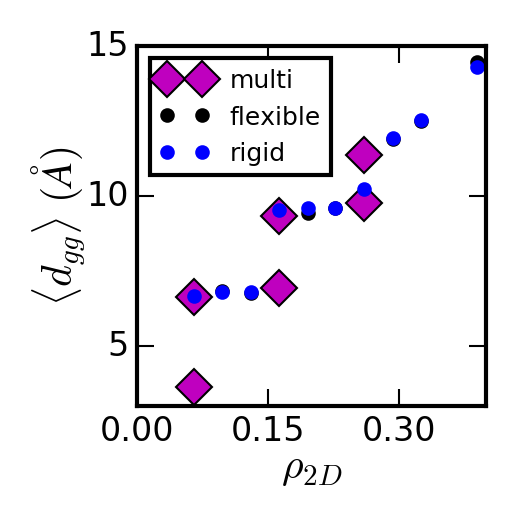
\includegraphics[trim={0.35cm 0.25cm 0.05cm 0.05cm},clip,width=.39\textwidth]{d_gg}
%		\end{subfigure}
		\caption{\textit{Plot of average graphene-graphene separation as a function of 2D-number density.} Multi refers to the instances in the flexible case where coexistence between multiple numbers of water layers was observed.}
		\label{fig:dgg_1}
	\end{figure}
	
	The transitions between states with different number of layers occur for both rigid and flexible graphene at the same values of \(\rho_{2D}\), however they are qualitatively different. The rigid case is characterized by discontinuous ML-BL, and BL-TL transitions, although the latter seems more gradual than the former. Further work focusing on this transition is required to establish unequivocally whether the BL-TL transition is continuous or discontinuous. In the case of flexible confinement, at the transitions we observe a split in the \(d_{gg}\) distances (shown as pink diamonds in Figure \ref{fig:dgg_1}). Upon closer inspection, we observe the coexistence of an n-layer and an (n+1)-layer state in the same system, spatially separated by an interface (Fig. \ref{fig:dgg_2}). We observe the split even for low density ML (Fig. \ref{fig:dgg_2}a), where the strong graphene adhesion helps forming pockets of ice, similarly to the phenomena observed in Ref.~\citenum{Algara-Siller2015}. The heat maps in Figure \ref{fig:dgg_2} show the position of water as a function of \(d_{gg}\) averaged over time. The nL/(n+1)L coexisting states are particularly clear in these plots.  
	
	\begin{figure}[ht!]
		\centering
		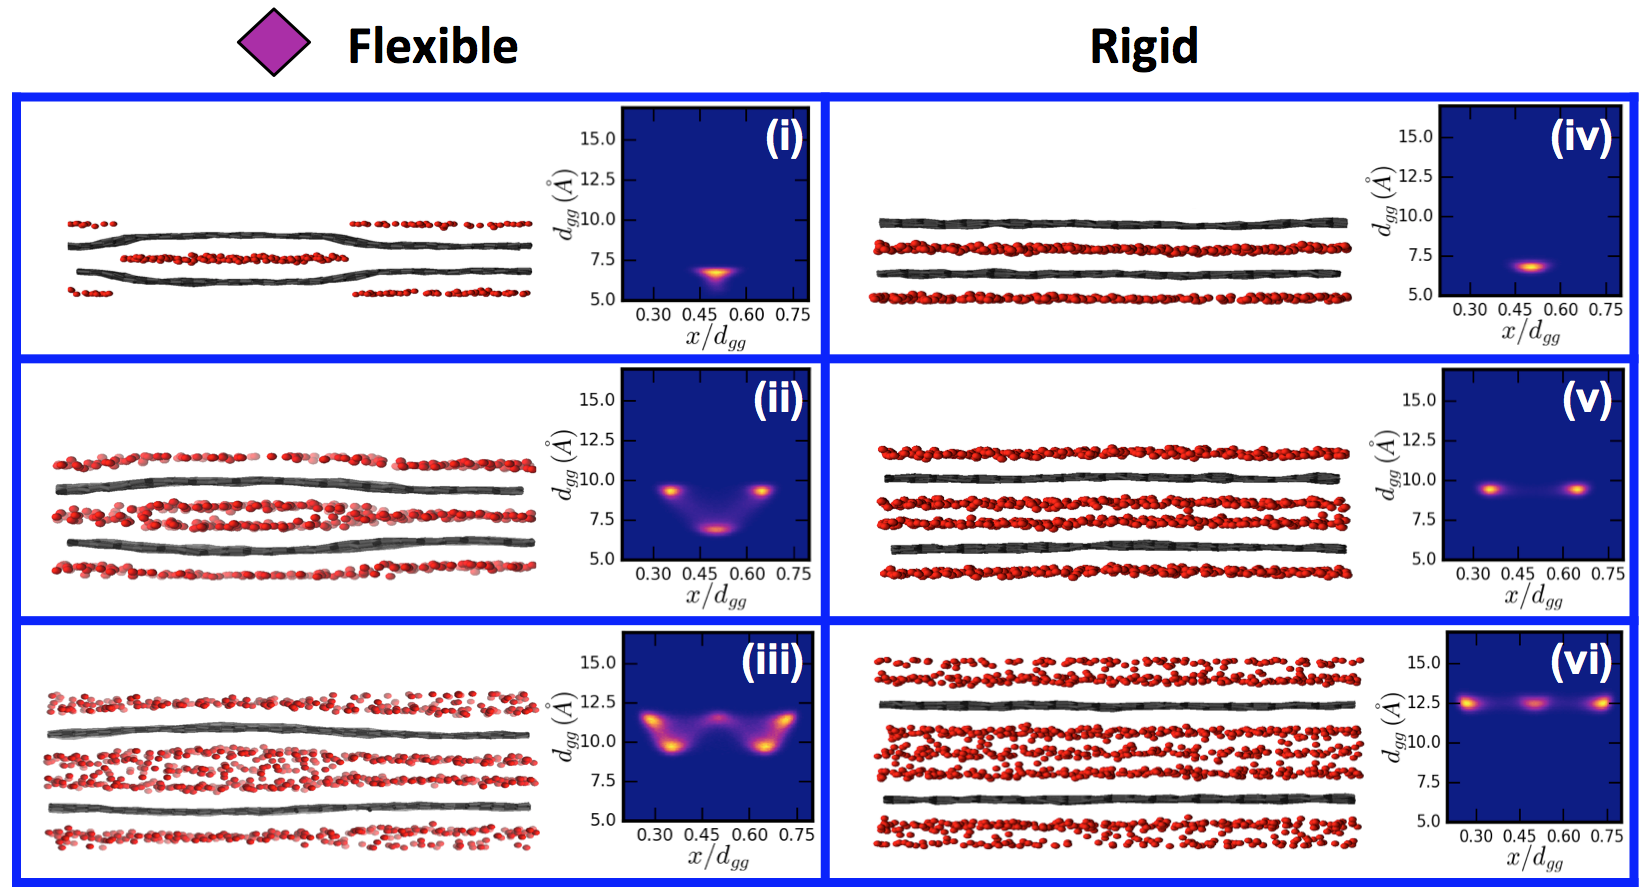
\includegraphics[width=.89\textwidth]{dgg_snaps7}
		\caption{\textit{Snapshots of out-of-plane water layering and heatmap of water location and graphene-graphene separation.} Left panels correspond to flexible systems, and right panels correspond to rigid systems. \textbf{Snapshots.} Water-graphene systems as a function of increasing 2D-density, water oxygens are red, graphene carbons are grey and water hydrogens are not displayed for clarity. \textbf{Heatmaps.} 2D histogram of the distance of water to a reference wall versus the graphene-graphene separation distance, warmer colors representing a higher number of observations.}
		\label{fig:dgg_2}
	\end{figure}
	
	The incommensurability of the systems at the transition points is evidenced by a broadening of the density peaks at \(\rho_{2D}\)=0.245, in the BL-TL transition illustrated in Figure \ref{fig:dgg_2_to_3}. The heat maps reveal two broad peaks in the case of rigid confinement and a split between BL and TL in the case of flexible graphene. Additionally at the \(\rho_{2D}\) depicted (0.245), the graphene separation for the rigid system falls between the split of the analogous flexible case (Fig \ref{fig:dgg_1}).
	
	\begin{figure}[ht!]
		\centering
		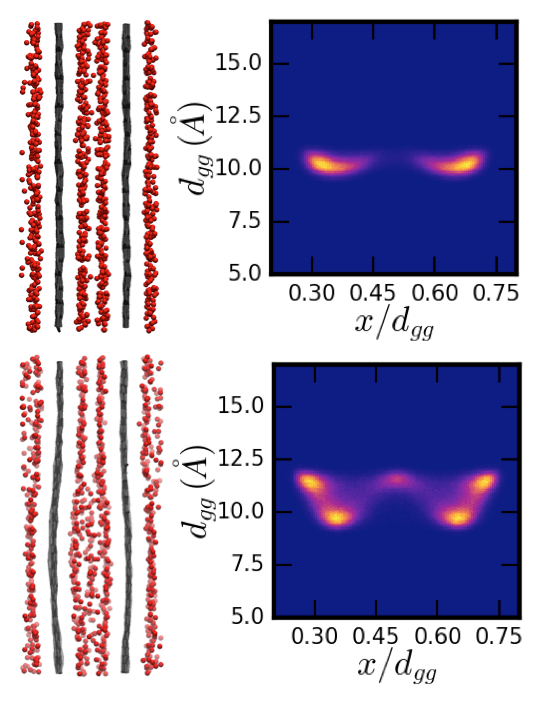
\includegraphics[width=0.49\textwidth]{d12_smearing} %
		\caption{\textit{Snapshots of out-of-plane water layering and heatmap of water location and graphene-graphene separation for bilayer to trilayer transition.} (a,c) Water-graphene systems as a function of increasing 2D-density, water oxygens are red, graphene carbons are grey and water hydrogens are not displayed for clarity. Images not drawn to size. (b,d) 2D histogram of the distance of water to a reference wall versus the graphene-graphene separation distance, warmer colors representing a higher number of observations. (a-b) Represent flexible system, (c-d) represent rigid system.}
		\label{fig:dgg_2_to_3}
	\end{figure}
	
	%%%%%%%%%%%%%%%%%%%%%%%%%%%%%%%%%%%%%%%%
	%%%%%%%%%%%%%%%%%%%%%%%%%%%%%%%%%%%%%%%%

\subsection{In-plane structure}

Besides the transitions between multi-layered states as \(\rho_{2D}\) is increased, full characterization of the state of water under confinement requires assessing the in-plane structure and dynamics, so that we can discern between ice, liquid, gas, or more complex phases such as glass or heterogeneous liquids. For this purpose, we calculate the oxygen-oxygen pair correlation function \(g_{OO}(R)\), the 3-body angle distributions between the oxygen atoms of coplanar water molecules, \(p(\theta\)), and the lateral mean-squared-displacement, \(MSD_{||}\), for all the cases. To calculate \(g_{OO}(R)\), the oxygen atoms were histogrammed into 0.6\r A bins according to their x-coordinate. The RDF was calculated for each bin, and the average of all bins is the \(g_{OO}(R)\). For the 3-body angle distributions, the angle \(\theta\) is the angle between the oxygen and the first and second nearest neighbors within the same bin. We estimate the lateral diffusion coefficient, \(\mathcal{D}_{||}\), from the lateral MSD using Einstein's relation.

We start by analyzing the phase behavior in the ML state, which spans from \(\rho_{2D}=0.062\) to \(\rho_{2D}=0.123\) and 6 \r A < \(d_{gg}\) < 8 \r A (Figure \ref{fig:struct_6_7_8}). For the lowest density investigated \(\rho_{2D}=0.062\), there is not enough water to form a full monolayer. In the rigid case this leads to liquid-vapor coexistence. We assign the liquid label because of the relatively high diffusivity of 2.26, reported in Figure \ref{fig:msd}a, which is close to bulk water. It is important to note, however, that the monolayer liquid does not resemble structurally bulk water characterized by tetrahedral order. The \(p(\theta\)) in this case reveals a peak at \(\sim\)104 degrees, similarly to bulk water, but also a smaller peak around 120 degrees. The RDF of this ML-liquid phase is also substantially more structured than bulk water. For \(\rho_{2D}=0.062\), the flexible system forms pockets of square and rhombic ice (Fig \ref{fig:ice_figs}a), characterized by peaks in \(p(\theta\)) at \(\sim\)90 and 160 degrees. The snapshot of the system reveals a region where there is no water, but unlike the rigid \(\rho_{2D}=0.062\) system, this area is not a vapor region, but a region of graphene-graphene contact (Fig \ref{fig:dgg_2}a), there is no water vapor in the flexible system. The diffusivity is 4 orders of magnitude lower in the flexible case. When the density is increased to 0.092 and 0.123, for the rigid case Figure \ref{fig:gr_ang_6_7_8_r}, the \(g_{OO}(R)\) become substantially more structured, and the \(p(\theta\)) are characterized by a bimodal distribution with peaks at 90 and 160 degrees, representative of square and rhombic ice respectively. Close up snapshots of these ice structures are shown in Figure \ref{fig:ice_figs}a. The appearance of ice is also confirmed by the self-diffusion coefficients. At \(\rho_{2D}=0.092\) the ice phase coexists with a vapor phase, while the vapor phase practically vanishes at \(\rho_{2D}=0.123\). The flexible case is very similar to the rigid confinement for \(\rho_{2D}=0.123\), where ML-ice forms. However, at \(\rho_{2D}=0.123\) the system resembles the liquid-vapor coexistence observed for the rigid case at \(\rho_{2D}=0.062\). In summary, for the ML states, at \(\rho_{2D}=0.123\), before the transition to the BL, both rigid and flexible systems behave very similarly, displaying phases of ML-ice. For \(\rho_{2D}=0.062\) the rigid system shows a ML-liquid-vapor phase, and the flexible system displays pockets of ML-ice between graphene-graphene contacts. For \(\rho_{2D}=0.092\), the flexible systems exhibit a ML-liquid-vapor phase, and the rigid systems exhibit a ML-ice-vapor coexistence. 
	
The results of the analysis for the BL states are shown in Figure \ref{fig:struct_9_10_11}. The BL regime spans from \(\rho_{2D}=0.154\) to \(\rho_{2D}=0.215\) and 8 \r A < \(d_{gg}\) < 10 \r A. For the rigid case, the coexistence of ice and vapor is observed for \(\rho_{2D}=0.154\) and \(\rho_{2D}=0.185\). In contrast to the ML-ice, the BL-ice phase displays AA stacking hexagonal structure with an abundance of defects necessary to accommodate the nearly circular vapor-solid interface in the rectangular simulation box (Fig. \ref{fig:ice_figs}b). This is confirmed by the enhanced structure of the \(g_{OO}(R)\) plots in Fig \ref{fig:gr_ang_9_10_11_r}, which exhibit a smooth oscillatory structure, higher than bulk water and qualitatively different from the structure of square ice. Additionally, the peak of \(p(\theta\)) has shifted to \(\sim\)114 and the shoulder at 160 has vanished. As \(\rho_{2D}\) is increased to 0.215, the amount of water confined is too large to develop in-plane crystalline order, and the water adopts a liquid phase, with small patches of ice nucleating and dissipating constantly. This effect is reflected in the lower-than-liquid self-diffusion coefficient, and in the shoulder at \(\theta\simeq140\) in the \(p(\theta\)) distribution. These ice nucleation events suggest that we are close to the solid-liquid phase transition. In the flexible case, for \(\rho_{2D}=0.154\) we have ML-liquid and BL-liquid coexisting, as observed from simulation snapshots (Fig \ref{fig:gr_ang_9_10_11_f}. These coexisting phases are also structurally different, as confirmed by their \(g_{OO}(R)\) and \(p(\theta\)) plots. Although there are structural differences between the n=1 and n=2 regions of the system, the interface between the two prevents any solidification of the n=1 component, and the resulting \(D_{||}\) is similar to the other BL-liquid systems studied. At higher densities, the system transitions to the BL state. The water phase in the BL states is very similar to that observed for rigid confinement when \(\rho_{2D}=0.215\), namely BL-liquid. The diffusivity when \(\rho_{2D}=0.215\) is slightly higher in the flexible case.

As we increase the density beyond 0.245, the systems transition into the TL state and subsequently into 4+ layer states, where the differences between rigid and flexible systems are minor. Under our simulations conditions, the water in the TL state is in liquid phase, for both rigid and flexible systems, even the layers close to the confining surfaces. The only difference between flexible and rigid confinement for the TL state is the higher self-diffusion coefficients in the former case. But all converge towards bulk liquid at large densities. The analysis for the TL states is in good agreement with previous studies (Ref.~\citenum{Mosaddeghi2012}).

\setlength{\fboxsep}{0.75pt}%
\setlength{\fboxrule}{1.2pt}%

\begin{figure}[ht!]
	\centering
	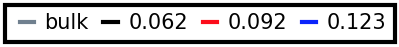
\includegraphics[width=0.46\textwidth]{leg_bulk_6_7_8}\\
  \fbox{\begin{subfigure}[b]{0.47\textwidth}
    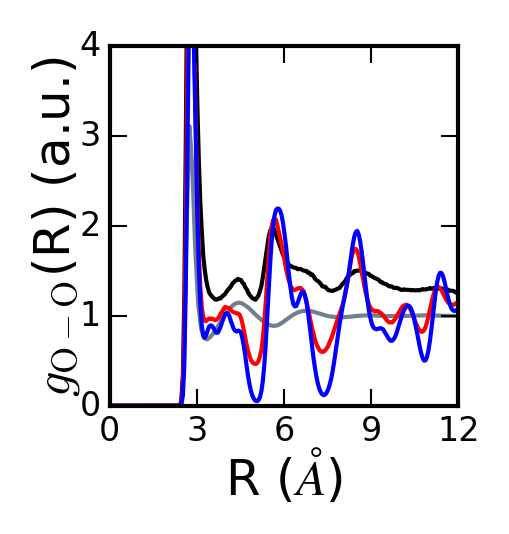
\includegraphics[trim={0.05cm 0.30cm 0.25cm 0.15cm},clip,width=0.46\textwidth]{g_r_2D_6_7_8_r}
    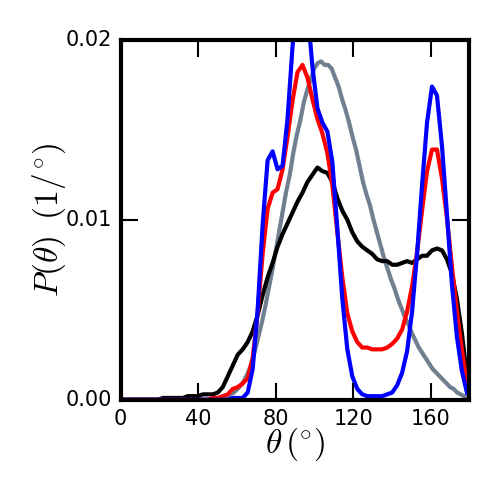
\includegraphics[trim={0.25cm 0.25cm 0.05cm 0.15cm},clip,width=0.485\textwidth]{ang_3B_6_7_8_r} 
     \fbox{\includegraphics[width=0.29\textwidth]{6A_r0} 
             	\llap{\raisebox{-0.4cm}{\color{white} \small  \fcolorbox{black}{black}{\(\mathcal{D}_{||}=2.26\)}}}}
     \fbox{\includegraphics[width=0.29\textwidth]{7A_r0}
     		\llap{\raisebox{-0.4cm}{\color{white} \small  \fcolorbox{red}{red}{\(\mathcal{D}_{||}=5.4e\scalebox{0.75}[1.0]{\( - \)}3\)}}}}
     \fbox{\includegraphics[width=0.29\textwidth]{8A_r0}
     		\llap{\raisebox{-0.4cm}{\color{white} \small  \fcolorbox{blue}{blue}{\(\mathcal{D}_{||}=1.4e\scalebox{0.75}[1.0]{\( - \)}4\)}}}}
    \caption{}
    \label{fig:gr_ang_6_7_8_r}
  \end{subfigure}}
  \fbox{\begin{subfigure}[b]{0.47\textwidth}
    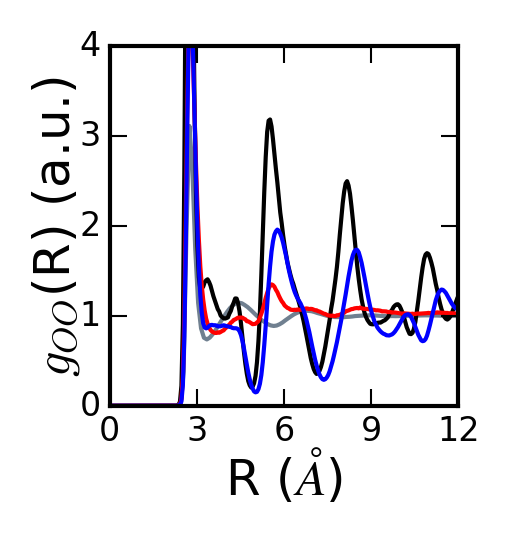
\includegraphics[trim={0.05cm 0.30cm 0.25cm 0.15cm},clip,width=0.46\textwidth]{g_r_2D_6_7_8_f}
    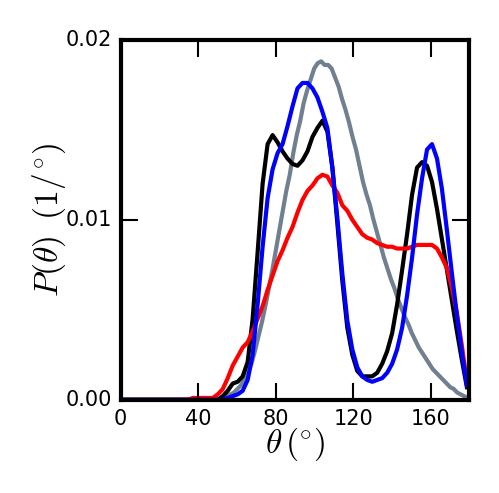
\includegraphics[trim={0.25cm 0.25cm 0.05cm 0.15cm},clip,width=0.485\textwidth]{ang_3B_6_7_8_f}
     \fbox{\includegraphics[width=0.29\textwidth]{6A_f0}
     		\llap{\raisebox{-0.4cm}{\color{white} \small \fcolorbox{black}{black}{\(\mathcal{D}_{||}=3.2e\scalebox{0.75}[1.0]{\( - \)}4\)}}}} %\raisebox{1.8cm} for in upper right corner
     \fbox{\includegraphics[width=0.29\textwidth]{7A_f0}
     		\llap{\raisebox{-0.4cm}{\color{white} \small \fcolorbox{red}{red}{\(\mathcal{D}_{||}=3.35\)}}}}
     \fbox{\includegraphics[width=0.29\textwidth]{8A_f0}
     		\llap{\raisebox{-0.4cm}{\color{white} \small \fcolorbox{blue}{blue}{\(\mathcal{D}_{||}=1.3e\scalebox{0.75}[1.0]{\( - \)}2\)}}}}
    \caption{}
    \label{fig:gr_ang_6_7_8_f}
  \end{subfigure}}
	\caption{\textit{Monolayer lateral oxygen-oxygen pair correlation functions, three-body angle distributions, and snapshots of monolayer systems.} (\protect\subref{fig:gr_ang_6_7_8_r}) rigid systems, (\protect\subref{fig:gr_ang_6_7_8_f}) flexible systems.  \textbf{Top.} Distribution of water oxygen distances and distribution of intralayer 3B angle formed between and given oxygen and its 2 nearest neighbors. \textbf{Bottom.} Snapshots of systems from left to right: \(\rho_{2D}=\) 0.062, 0.092, 0.123. Oxygens are in red, hydrogens are in white and for clarity, only one interlayer of water is depicted, and the graphene sheets are not displayed. Lateral diffusion coefficients are given in units of \((m^2/s) \times 10^9\), in the colored box in the bottom right corner. The lowest density system of (\protect\subref{fig:gr_ang_6_7_8_f}) is comprised of a coexistence between different number of water interlayers, highlighted in black (n=0) and blue (n=1).}
	\label{fig:struct_6_7_8}
\end{figure}

\begin{figure}[ht!]
	\centering
	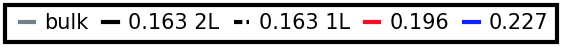
\includegraphics[width=0.60\textwidth]{leg_bulk_9_10_11}\\
  \fbox{\begin{subfigure}[b]{0.48\textwidth}
    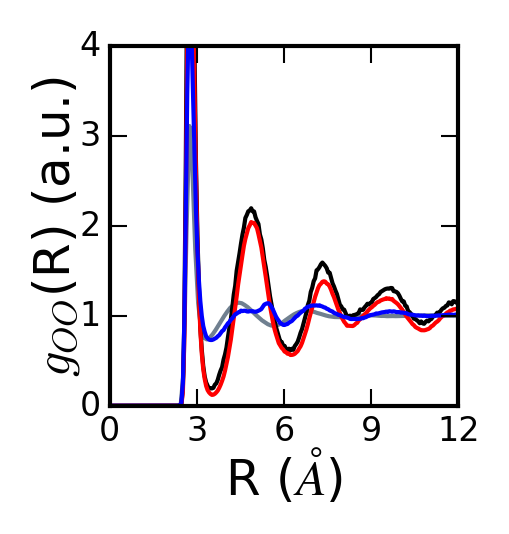
\includegraphics[trim={0.05cm 0.30cm 0.25cm 0.15cm},clip,width=0.46\textwidth]{g_r_2D_9_10_11_r}
    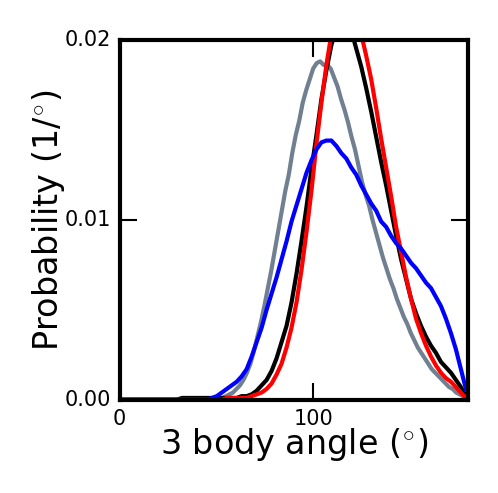
\includegraphics[trim={0.25cm 0.25cm 0.05cm 0.15cm},clip,width=0.485\textwidth]{ang_3B_9_10_11_r} 
     \fbox{\includegraphics[width=0.29\textwidth]{9A_r0}
     		\llap{\raisebox{-0.4cm}{\color{white} \small \fcolorbox{black}{black}{\(\mathcal{D}_{||}=2.2e\scalebox{0.75}[1.0]{\( - \)}2\)}}}}
     \fbox{\includegraphics[width=0.29\textwidth]{10A_r0}
     		\llap{\raisebox{-0.4cm}{\color{white} \small  \fcolorbox{red}{red}{\(\mathcal{D}_{||}=5.7e\scalebox{0.75}[1.0]{\( - \)}3\)}}}}
     \fbox{\includegraphics[width=0.29\textwidth]{11A_r0}
     		\llap{\raisebox{-0.4cm}{\color{white} \small  \fcolorbox{blue}{blue}{\(\mathcal{D}_{||}=1.07\)}}}}
    \caption{}
    \label{fig:gr_ang_9_10_11_r}
  \end{subfigure}}
  \fbox{\begin{subfigure}[b]{0.48\textwidth}
    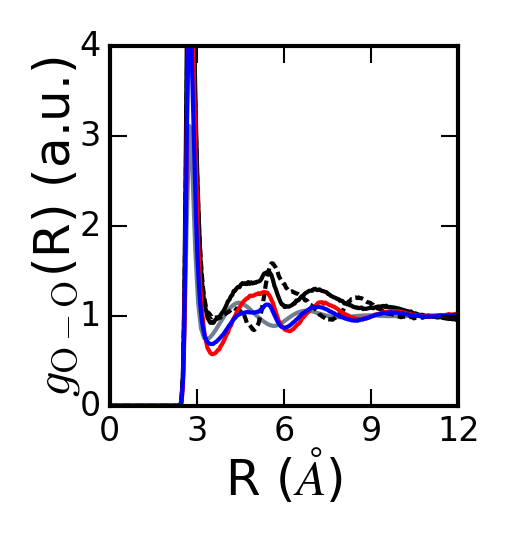
\includegraphics[trim={0.05cm 0.30cm 0.25cm 0.15cm},clip,width=0.46\textwidth]{g_r_2D_9_10_11_f}
    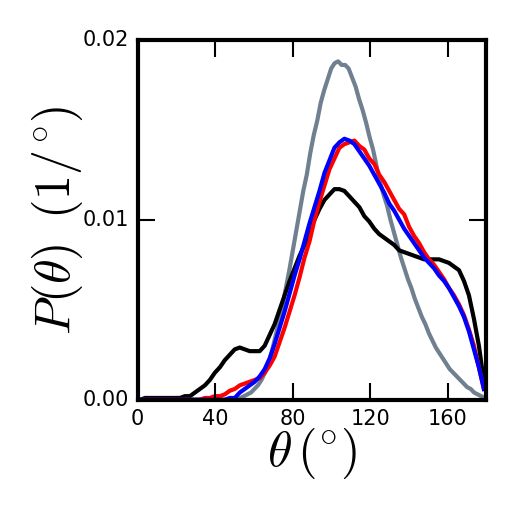
\includegraphics[trim={0.25cm 0.25cm 0.05cm 0.15cm},clip,width=0.485\textwidth]{ang_3B_9_10_11_f}
     \fbox{\includegraphics[width=0.29\textwidth]{9A_f0}
     		\llap{\raisebox{-0.4cm}{\color{white} \small  \fcolorbox{black}{black}{\(\mathcal{D}_{||}=1.79\)}}}}
     \fbox{\includegraphics[width=0.29\textwidth]{10A_f0}
     		\llap{\raisebox{-0.4cm}{\color{white} \small  \fcolorbox{red}{red}{\(\mathcal{D}_{||}=1.65\)}}}}
     \fbox{\includegraphics[width=0.29\textwidth]{11A_f0}
     		\llap{\raisebox{-0.4cm}{\color{white} \small  \fcolorbox{blue}{blue}{\(\mathcal{D}_{||}=1.22\)}}}}
    \caption{}
    \label{fig:gr_ang_9_10_11_f}
  \end{subfigure}}
	\caption{\textit{Bilayer lateral oxygen-oxygen pair correlation functions, three-body angle distributions, and snapshots of monolayer systems.} (\protect\subref{fig:gr_ang_9_10_11_r}) rigid systems, (\protect\subref{fig:gr_ang_9_10_11_f}) flexible systems. \textbf{Top.} Distribution of water oxygen distances and distribution of intralayer 3B angle formed between and given oxygen and its 2 nearest neighbors. \textbf{Bottom.} Snapshots of systems from left to right: \(\rho_{2D}=\) 0.154, 0.185, 0.215. Oxygens are in red, hydrogens are in white and for clarity, only one interlayer of water is depicted, and the graphene sheets are not displayed. Lateral diffusion coefficients are given in units of \((m^2/s) \times 10^9\), in the colored box in the bottom right corner. The lowest density system of (\protect\subref{fig:gr_ang_9_10_11_f}) is comprised of a coexistence between different number of water interlayers, highlighted in black (n=1) and blue (n=2).}
	\label{fig:struct_9_10_11}
\end{figure}

\begin{figure}[ht!]
	\centering
	\begin{subfigure}[b]{0.30\textwidth}
    		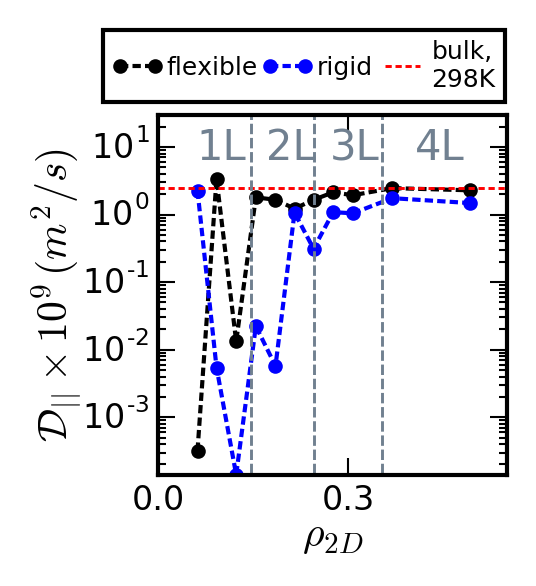
\includegraphics[trim={0.25cm 0.25cm 0.15cm 0.15cm},clip,width=0.99\textwidth]{diffusion_coeff_2D_f_r}
		\caption{}
    		\label{fig:diff}
   	\end{subfigure}	
	\begin{subfigure}[b]{0.28\textwidth}
    		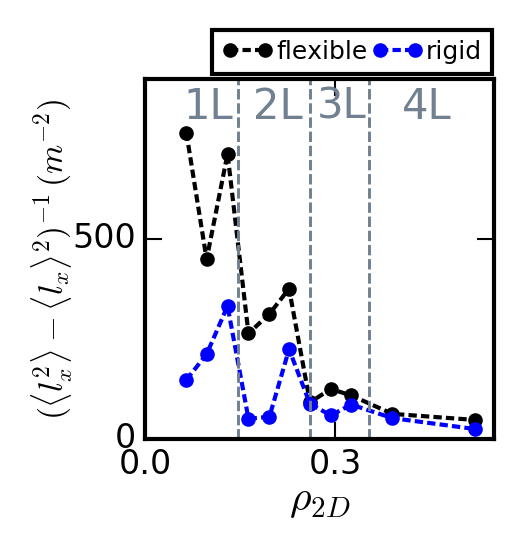
\includegraphics[trim={0.25cm 0.25cm 0.15cm 0.15cm},clip,width=0.99\textwidth]{compressibility}
		\caption{}
    		\label{fig:comp}
   	\end{subfigure}
	\caption{\textit{Comparison of dynamic properties}. (\protect\subref{fig:diff}) The self-diffusion coefficient as a function of number density for the diffusion parallel to the graphene walls. (\protect\subref{fig:comp}) Fluctuations in the out-of-plane distance as an approximation of system compressibility.}
	\label{fig:msd}
\end{figure}

\begin{figure}[ht!]
	\centering
	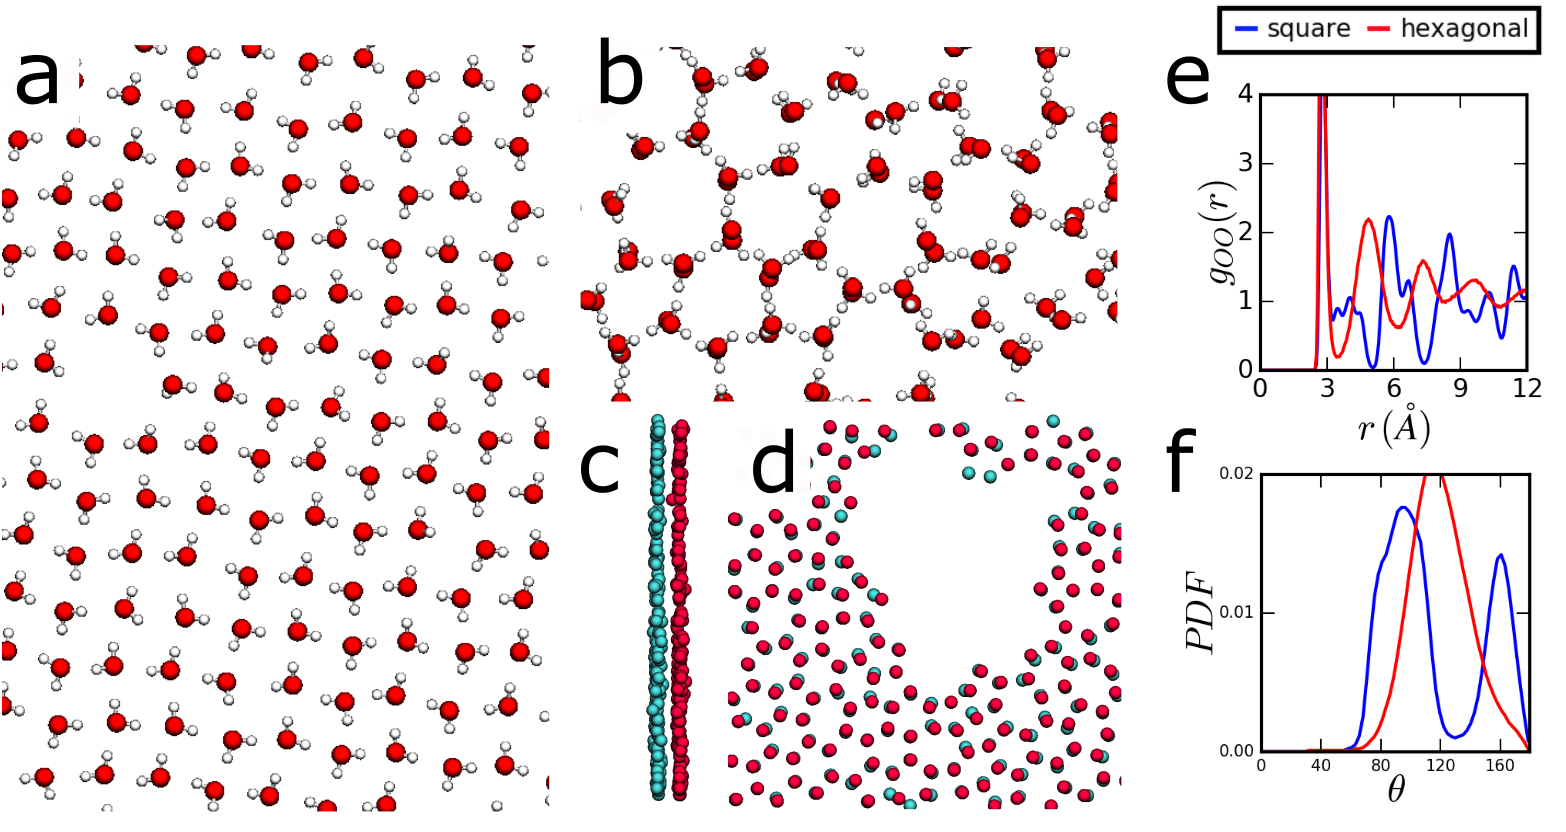
\includegraphics[width=.75\textwidth]{ices_all}
	\caption{\textit{Ice forms observed.} Oxygens are in red and cyan, hydrogens are in white. (a) Square and off-square ice observed in the following monolayer systems: \(\rho_{2D}=\)0.062 (flexible), \(\rho_{2D}=\)0.092 (rigid), \(\rho_{2D}=\)0.123 (both). (b-d) Hexagonal ice, observed in \(\rho_{2D}=\)0.154 and 0.185 (rigid). (b) a snapshot of the in-plane ordering. (c-d) the A-A stacking between layers is highlighted by depicting the oxygens of each layer in red and cyan. Hydrogens are not pictured. (e) \(g_{OO}(R)\) of square and hexagonal ice. (f) \(p(\theta)\) of square and hexagonal ice.}
	\label{fig:ice_figs}
\end{figure}

\clearpage
%%%%%%%%%%%%%%%%%%%%%%%%%%%%%%%%%%%%%%%%
%%%%%%%%%%%%%%%%%%%%%%%%%%%%%%%%%%%%%%%%
%%%%%%%%%%%%%%%%%%%%%%%%%%%%%%%%%%%%%%%%
%%%%%%%%%%%%%%%%%%%%%%%%%%%%%%%%%%%%%%%%
\section{Computational Methods}
	
	The model system consists of two parallel graphene sheets with water molecules filling the two interlayer spacings at a prescribed density \(\rho_{2D}\). The confinement occurs in the x-direction, and the in-plane dimensions of the system are \(L_y\) = 46.2 \r A, and  \(L_z\) = 48.5 \r A. Periodic boundary conditions are applied in all dimensions. We use the TIP4P-Ew model of water \cite{Horn2004}, and the parameters for graphene have been adapted from previous works \cite{Hummer2001,Patra2009}. All the bonded parameters are summarized in Table \ref{table:ff_parms}, and the non-bonded parameters in Table \ref{table:ff_parms_atoms}. 
	
	\begin{table}[ht!]
		\caption{\textit{Force field bonded parameters used for graphene in confined water simulations.}}
		\label{table:ff_parms}
		\centering
		\begin{tabular}{  l |  l l l } \hline
			\textbf{bonded term}  &\multicolumn{3}{c}{\textbf{parameters}} \\ \hline
			Bond  & \(K_b\)  (\(kCal/mol/\angstrom^2\))      & b\textsubscript{0}  (\r A)  &  \\ %\hline
			   & 938.0         & 1.40            &    \\   \hline
			Angle & \(K_{\theta}\)  (\(kCal/mol/rad^2\)) & \(\theta_0\) (degrees)   &          \\ 
			  & 126.0         & 120.0           &         \\ \hline
			Improper   & K\textsubscript{im} (kCal/mol)       & \(\chi_0\) (degrees)     &          \\ 
			 & 15.0          & 0.0             &          \\ \hline
			Dihedral      & K\textsubscript{di} (kCal/mol)       & n (multiplicity) & \(\phi\) (degrees)\\ 
			 & 3.150         & 2               & 180.0  \\  \hline
		\end{tabular}
	\end{table}
	
	\begin{table}[ht!]
		\caption{Force field parameters used for each atom type in confined water simulations.}
		\label{table:ff_parms_atoms}
		\begin{tabular}{ c|r|r|r}
			\hline
			\textbf{atom type} & \multicolumn{1}{c|}{\textbf{\begin{tabular}[c]{@{}c@{}}partial charge\\ (e)\end{tabular}}} & \multicolumn{1}{c|}{\textbf{\begin{tabular}[c]{@{}c@{}}\(\sigma\)\\ (\r A)\end{tabular}}} & \multicolumn{1}{c}{\textbf{\begin{tabular}[c]{@{}c@{}}\(\epsilon\)\\ (kCal/mole)\end{tabular}}} \\ \hline
			Graphene carbon & 0.0000  & 3.55 & 0.07   \\ 
			Water oxygen       & -1.0484 & 3.16435  & 0.16275  \\ 
			Water hydrogen   & 0.5242  & 0.00000 & 0.00000  \\ \hline
		\end{tabular}
	\end{table}

	All the simulations were performed with the LAMMPS software package \cite{Plimpton1995}. We use a time step of 2.0 fs for all the simulations, and all the simulations are performed at T = 298 K. We use the SHAKE algorithm \cite{Andersen1983} with a tolerance of 10\textsuperscript{-4} to keep the water molecules rigid, according to the TIP4P-Ew water model \cite{Horn2004}. Initially, we relax the system at constant volume in two steps. First, to get rid of close contacts or other high-energy configurations in the system, we run Brownian dynamics \cite{Schneider1978} for a short 10 ps where we limit the atoms displacement in a single time step to 0.1 \r A. After that, we simulate the system in the NVT ensemble for another 10 ps using a temperature damping parameter of 0.1 ps. After relaxing the system at constant volume, we perform runs of 10 ns in the NpT ensemble, where only the x-direction (i.e. the direction of confinement) is allowed to fluctuate, \(p_{xx}\) = 0.1 MPa. The temperature and pressure control were implemented using a Nos\' e-Hoover extended Lagrangian procedure \cite{Martyna1994} with characteristic damping times 0.1 and 1.0 ps, respectively. We consider the first 3 ns equilibration, and we collect data for analysis every 500 steps (2 ps) over the last 7 ns of the NpT trajectories. In the rigid cases, the graphene sheets are kept rigid but their center of mass position can fluctuate. In the flexible cases the full force-field is employed without further constraints.


%%%%%%%%%%%%%%%%%%%%%%%%%%%%%%%%%%%%%%%%%%%%%%%%%%%%%%%%%%%%%%%%%%%%%
%% The "Acknowledgement" section can be given in all manuscript
%% classes.  This should be given within the "acknowledgement"
%% environment, which will make the correct section or running title.
%%%%%%%%%%%%%%%%%%%%%%%%%%%%%%%%%%%%%%%%%%%%%%%%%%%%%%%%%%%%%%%%%%%%%
\begin{acknowledgement}

Please use ``The authors thank \ldots'' rather than ``The
authors would like to thank \ldots''.

\end{acknowledgement}

%%%%%%%%%%%%%%%%%%%%%%%%%%%%%%%%%%%%%%%%%%%%%%%%%%%%%%%%%%%%%%%%%%%%%
%% The same is true for Supporting Information, which should use the
%% suppinfo environment.
%%%%%%%%%%%%%%%%%%%%%%%%%%%%%%%%%%%%%%%%%%%%%%%%%%%%%%%%%%%%%%%%%%%%%
\begin{suppinfo}

A listing of the contents of each file supplied as Supporting Information
should be included. For instructions on what should be included in the
Supporting Information as well as how to prepare this material for
publications, refer to the journal's Instructions for Authors.

The following files are available free of charge.
\begin{itemize}
  \item Filename: brief description
  \item Filename: brief description
\end{itemize}

\end{suppinfo}

%%%%%%%%%%%%%%%%%%%%%%%%%%%%%%%%%%%%%%%%%%%%%%%%%%%%%%%%%%%%%%%%%%%%%
%% The appropriate \bibliography command should be placed here.
%% Notice that the class file automatically sets \bibliographystyle
%% and also names the section correctly.
%%%%%%%%%%%%%%%%%%%%%%%%%%%%%%%%%%%%%%%%%%%%%%%%%%%%%%%%%%%%%%%%%%%%%
\bibliography{references}

\end{document}
